\section{Regularization}

\subsection{}

\begin{frame}
    \frametitle{Underfitting and overfitting}

    \begin{alertblock}{Danger!}
        Neural networks are hard to fit, and real-life data are noisy.
        \emph{Underfitting} and \emph{overfitting} are your two biggest obstacles.
    \end{alertblock}
    \vspace{1ex}

    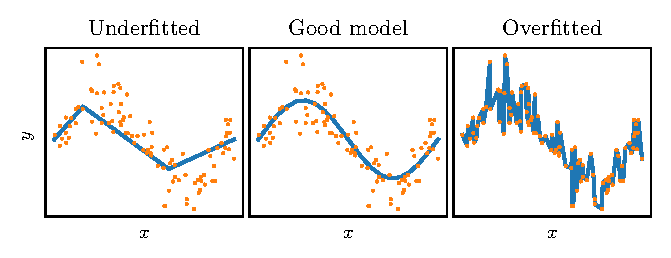
\includegraphics{under_over_train}
    \pause

    \begin{itemize}
        \item Underfitting: didn't train enough for the model to capture the underlying behavior
        \item Overfitting: training so good that neural network memorizes the data, including underlying noise
        \begin{itemize}
            \item Recall: with enough parameters, neural networks learn anything
        \end{itemize}
    \end{itemize}
\end{frame}

\begin{frame}
    \frametitle{Train, validate, test}

    Usual trick: split data into disjoint \textcolor{blue}{training} and \textcolor{Green4}{testing} sets
    \begin{itemize}
        \item Anywhere from 95/5 to 75/25 split is common
        \item Train \emph{only} on the \textcolor{blue}{training set}
        \item Periodically check loss of NN on \textcolor{Green4}{test set}
        \begin{itemize}
            \item Optimizer never sees test set: test set is honest check on NN fidelity
        \end{itemize}
    \end{itemize}
    \pause

    More advanced: split into disjoint \textcolor{blue}{training}, \textcolor{orange}{validation}, and \textcolor{Green4}{testing} set
    \begin{itemize}
        \item Aside on terminology
        \begin{itemize}
            \item Weights \& biases are \alert{parameters}---iteratively improved
            \item Design choices (\# layers, \# neurons, optimizer, \# epochs, etc.) are \alert{hyperparameters}---selected by ML designer
        \end{itemize}
        \item Select different sets of hyperparameters; for each:
        \begin{itemize}
            \item Train only on \textcolor{blue}{training set}, as before
            \item Compute validation loss on \textcolor{orange}{validation set}
        \end{itemize}
        \item Pick hyperparameters with lowest validation loss
        \item Then re-evaluate loss on \textcolor{Green4}{test data}
        \begin{itemize}
            \item Helps remove effects of variance on validation loss
        \end{itemize}
    \end{itemize}
\end{frame}

\begin{frame}
    \frametitle{Training loss vs.\ test loss}
    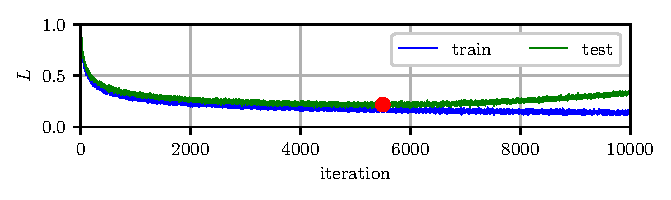
\includegraphics{loss}

    General pattern
    \begin{itemize}
        \item Modulo minor stochastic fluctuations, training loss should monotonically decrease: NN gets better at learning data
        \item Test loss usually at least slightly larger than training loss
        \begin{itemize}
            \item Because optimizer minimizes training loss but never sees test data
        \end{itemize}
        \item At some point, test loss increases: NN overfits to training data
        \item \alert{Early stopping}: use NN with minimum test loss
    \end{itemize}
\end{frame}

\begin{frame}
    \frametitle{Some regularization techniques (1/2)}

    \begin{block}{}
        Regularization: modifications that reduce generalization error
    \end{block}

    \begin{itemize}
        \item<+-> Early stopping
        \item<+-> Don't make NNs too big
        \begin{itemize}
            \item Rule of thumb: $\text{\# parameters} \le \text{\# data}$
        \end{itemize}
        \item<+-> $L^2$ regularization: use loss $\hat{L}(\y, \f(\x; \THETA)) = L(\y, \f(\x; \THETA)) + \alpha \|\THETA\|_2^2$
        \begin{itemize}
            \item Reduces weights, especially in directions that affect $L$ little
        \end{itemize}
        \item<+-> $L^1$ regularization: use loss $\hat{L}(\y, \f(\x; \THETA)) = L(\y, \f(\x; \THETA)) + \alpha \|\THETA\|_1$
        \begin{itemize}
            \item Promotes sparsity in $\THETA$
        \end{itemize}
        \item<+-> Add noise to NN input during training \citep{SietsmaNN91}
        \begin{itemize}
            \item Very non-intuitive to engineers
            \item Prevents overfitting: ``fuzzes'' out bad data
        \end{itemize}
        \item<+-> Bagging (bootstrap aggregating) \citep{BreimanML94}
        \begin{itemize}
            \item For data of size $n$, draw $d$ samples with replacement $m$ times
            \item Train one NN on each of the $m$ sets \& average results
        \end{itemize}
    \end{itemize}
\end{frame}

\begin{frame}
    \frametitle{Some regularization techniques (2/2)}
    \begin{itemize}
        \item<+-> \alert{Dropout} \citep{SrivastavaJMLR14}
        \begin{itemize}[<.->]
            \item During \textcolor{Green4}{training}, randomly remove some portion of connections
            \item Often 20\% of inputs and 50\% of hidden connections
            \item<+-> Put all connections back \& scale accordingly during \textcolor{blue}{inference}
            \item<+-> Motivation: kind of like bagging, but much cheaper
            \item With $n \gg 1$ iterations, essentially average of $n$ models
            \item One of the best regularization techniques; use it!
        \end{itemize}
    \end{itemize}

    \begin{tikzpicture}[node distance=3mm]
    \dropoutnetwork{green}

    \foreach \i/\j in {
        0/1, 0/3, 0/4, 1/0, 1/1, 1/2, 1/4, 2/0, 2/1, 2/2, 2/3, 2/4%
    } {
        \draw (input \i) -- (dense 0\j);
    }

    \foreach \i/\j in {
        0/0, 0/1, 0/2, 1/0, 1/1, 1/2, 1/3, 2/2, 3/0, 3/2, 4/0, 4/1, 4/2%
    } {
        \draw (dense 0\i) -- (dense 1\j);
    }

    \foreach \i/\j in {
        0/0, 1/0, 1/1, 2/1, 3/1%
    } {
        \draw (dense 1\i) -- (output \j);
    }
\end{tikzpicture}
%%% Local Variables:
%%% mode: latex
%%% TeX-master: "../nn"
%%% End:

    \hfill
    \begin{tikzpicture}[node distance=3mm]
    % Box.
    \draw [fill=green!10, rounded corners] (-0.75, -0.25) rectangle (1.75, 1.75);

    % Nodes.
    \node (input 0) [io mini] {};
    \node (input 1) [io mini, right=of input 0] {};
    \node (input 2) [io mini, right=of input 1] {};

    \node (dense 01) [neuron mini, above=of input 0] {};
    \node (dense 00) [neuron mini, left=of dense 01] {};
    \node (dense 02) [neuron mini off, right=of dense 01] {};
    \node (dense 03) [neuron mini off, right=of dense 02] {};
    \node (dense 04) [neuron mini off, right=of dense 03] {};

    \node (dense 10) [neuron mini off, above=of dense 00, xshift=2.5mm] {};
    \node (dense 11) [neuron mini, right=of dense 10] {};
    \node (dense 12) [neuron mini, right=of dense 11] {};
    \node (dense 13) [neuron mini off, right=of dense 12] {};

    \foreach \i in {0, 1} {
        \pgfmathtruncatemacro{\j}{\i + 1}
        \node (output \i) [io mini, above=of dense 1\j] {};
    }

    % Connections.
    \foreach \i in {0, 1} {
        \foreach \j in {0, ..., 2} {
            \draw (input \j) -- (dense 0\i);
        }

        \foreach \j in {1, 2} {
            \draw (dense 0\i) -- (dense 1\j);
        }
    }

    \foreach \i in {1, 2} {
        \foreach \j in {0, 1} {
            \draw (dense 1\i) -- (output \j);
        }
    }
\end{tikzpicture}
%%% Local Variables:
%%% mode: latex
%%% TeX-master: "../nn"
%%% End:

    \hfill
    \input{figures/dropout3}
    \hfill
    \uncover<2->{\begin{tikzpicture}[node distance=3mm]
    \dropoutnetwork{blue}

    \foreach \i in {0, ..., 4} {
        \foreach \j in {0, ..., 2} {
            \draw (input \j) -- (dense 0\i);
        }

        \foreach \j in {0, ..., 3} {
            \draw (dense 0\i) -- (dense 1\j);
        }
    }

    \foreach \i in {0, 1} {
        \foreach \j in {0, ..., 3} {
            \draw (dense 1\j) -- (output \i);
        }
    }
\end{tikzpicture}
%%% Local Variables:
%%% mode: latex
%%% TeX-master: "../nn"
%%% End:
}

    \begin{itemize}
        \item \alert{Batch normalization} \citep{IoffeICML15}
        \begin{itemize}
            \item Automatically shifts \& scales values to have mean 0 \& variance 1 for each mini-batch
            \item Results in better behavior and easier learning: inputs to activations won't fly to $\pm \infty$
        \end{itemize}
    \end{itemize}
\end{frame}

%%% Local Variables:
%%% mode: latex
%%% TeX-master: "../nn"
%%% End:
